\subsection{Casa Familia}

\begin{wrapfigure}{R}{0.4\textwidth}
\vspace{-35pt}
\hspace{-35pt}
\centering
   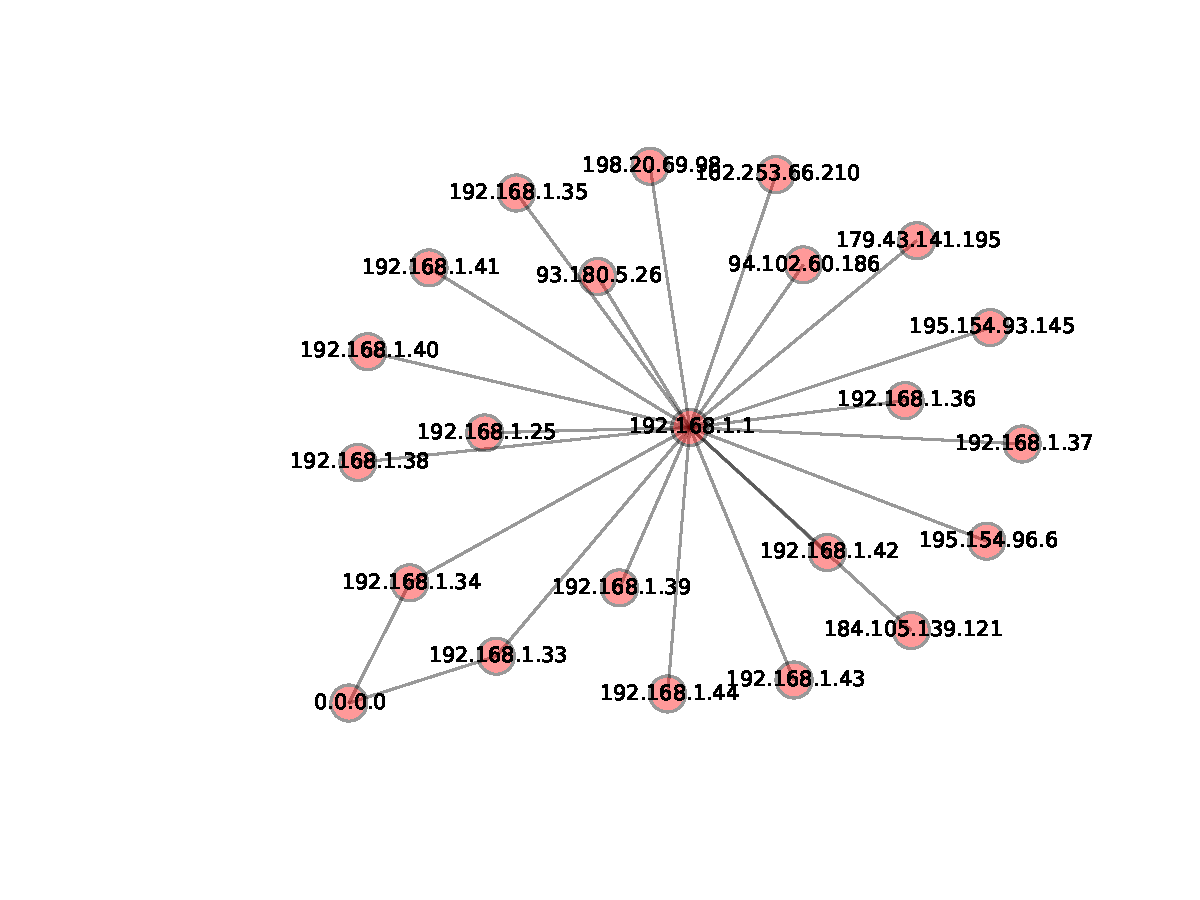
\includegraphics[width=0.4\textwidth]{resultados/casa/conectividadNX.pdf}
\vspace{-30pt}
   \caption{Grafo de la red}
\end{wrapfigure}

En el caso de la casa familiar sab\'iamos de antemano que la direcci\'on del router
es 192.168.1.1 y que 192.168.1.35 pertenece al dispositivo que m\'as tiempo estuvo
prendido, el mismo es una notebook. La ip del router es de las que aparece con mayor
frecuencia en los campos SRC o DST, mientras que $.35$ solo aparece un alto n\'umero
de veces en DST. 

Ambos grafos presentan forma de estrella, teniendo al router como centro. 
La entrop\'ia fue: $1.68$ para el modelo $SRC$ y $2.67$ para el modelo DST.
Cabe destacar que aunque no est\'a reflejado en los gr\'aficos, sucedi\'o algo interesante, 
aparecieron paquetes ARP con direcciones que no pertenecian a la red local.

\begin{figure}[H]
	\center
	\begin{subfigure}{0.4\textwidth}
		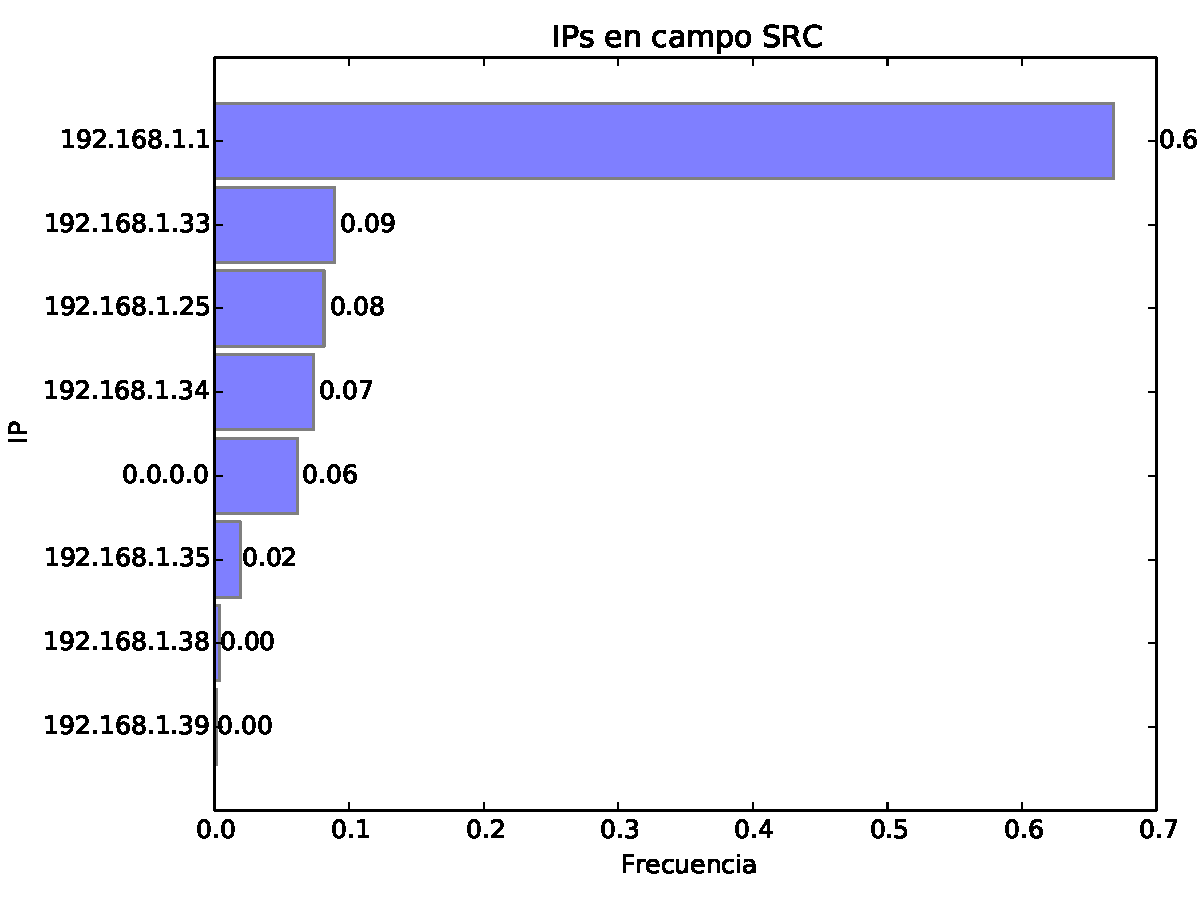
\includegraphics[width=1.0\textwidth]{resultados/casa/ipsSrc_1_6805902069.pdf}
		\caption{Estimaci\'on de la probabilidad de cada s\'imbolo en modelo SRC}
	\end{subfigure}
	~
	\begin{subfigure}{0.4\textwidth}
		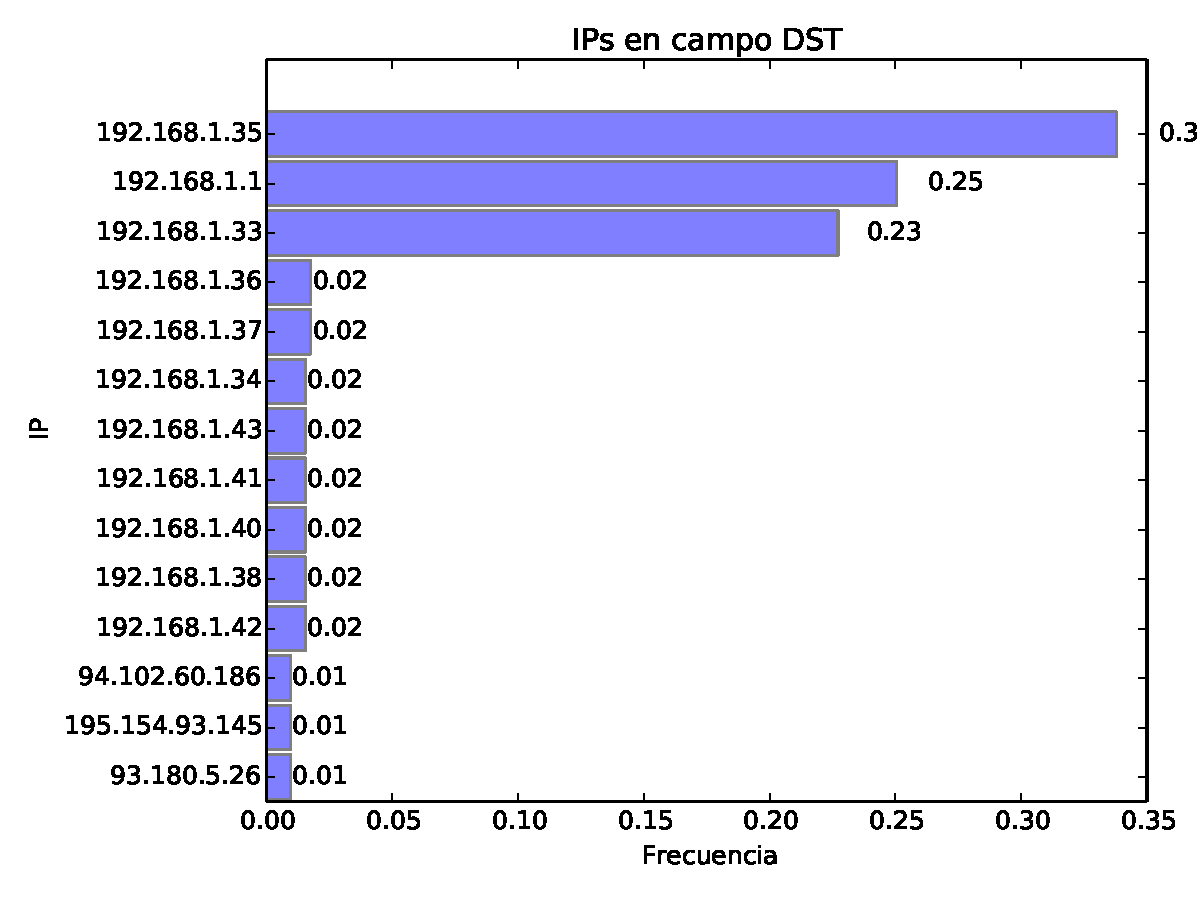
\includegraphics[width=1.0\textwidth]{resultados/casa/ipsDst_2_67355481854.pdf}
		\caption{Estimaci\'on de la probabilidad de cada s\'imbolo en modelo DST}
	\end{subfigure}
\end{figure}


\subsection{Starbucks}

\begin{wrapfigure}{R}{0.4\textwidth}
\vspace{-35pt}
\hspace{-35pt}
\centering
   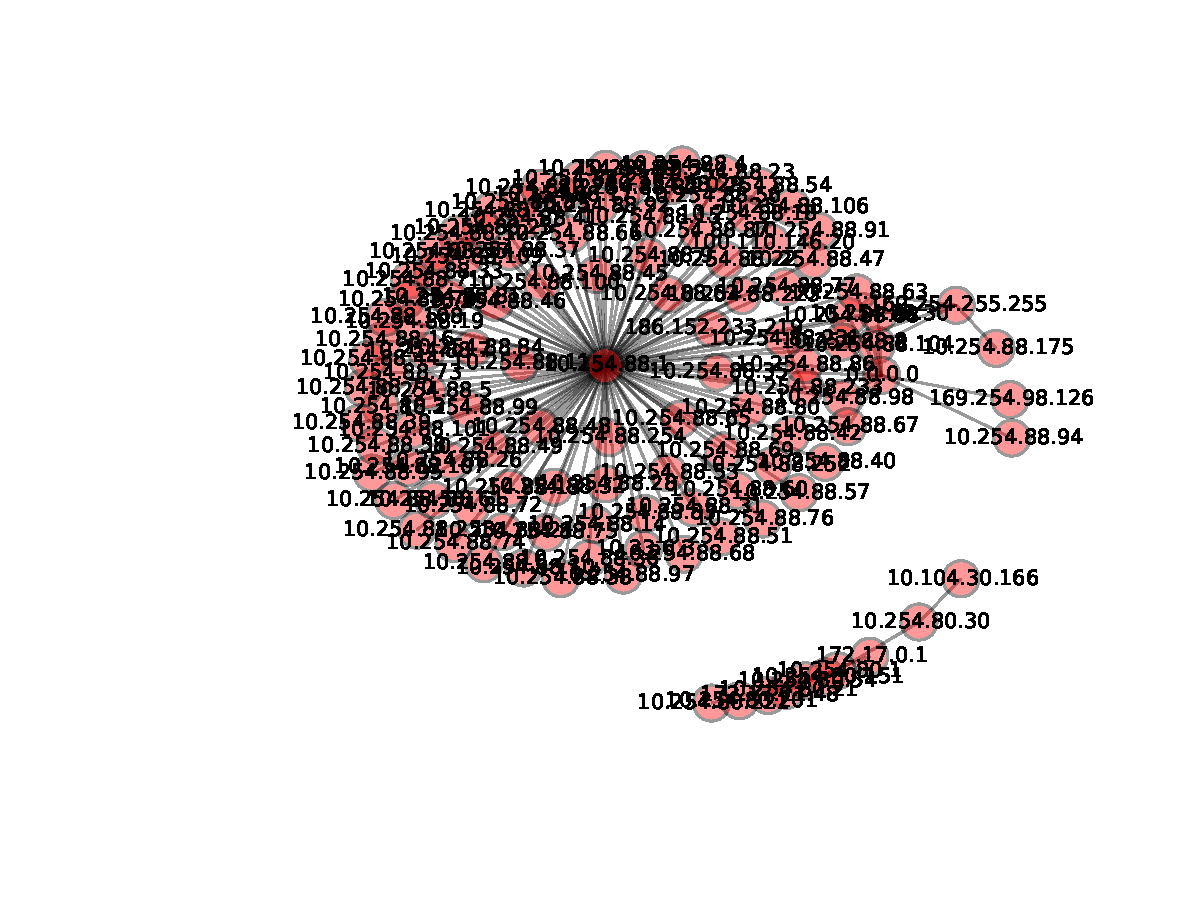
\includegraphics[width=0.4\textwidth]{resultados/starbucks/conectividadNX.pdf}
\vspace{-30pt}
   \caption{Grafo de la red}
\end{wrapfigure}


Para el caso de la red abierta disponible en Starbucks, podemos ver en el 
grafo simple una notoria centralizaci\'on de paquetes hacia/desde la direcci\'n
10.254.88.1, la cual a su vez posee una alta frecuencia de aparici\'on en ambos
modelos. Esto ser\'ia el comportamiento esperado del router de la red
10.254.88.0/24. Asumimos que \'esta es la direcci\'on de la red puesto que 
la mayor\'ia de las IPs de los paquetes capturados difieren en el \'ultimo octeto.
Por otro lado, podemos ver que la segunda direcci\'on con mayor frecuencia en DST
fue 10.254.80.1, seguida por 10.254.88.8. Suponemos que $88.8$ es la pc del lugar
dada la ip baja, y la cantidad de apariciones. Por otro lado, no sabemos que es
$80.1ç$ dado que parece formar una red aparte de la sniffeada.

La entrop\'ia fue: $4.61$ para el modelo $SRC$ y $3.76$ para el modelo
DST.


Nuevamente entre los paquetes capturados volvieron a aparecer direcciones que
no parecieran pertenecer a la red local, resultando sumamente interesante el caso
de 10.254.80.1

\begin{figure}[H]
	\center
	\begin{subfigure}{0.4\textwidth}
		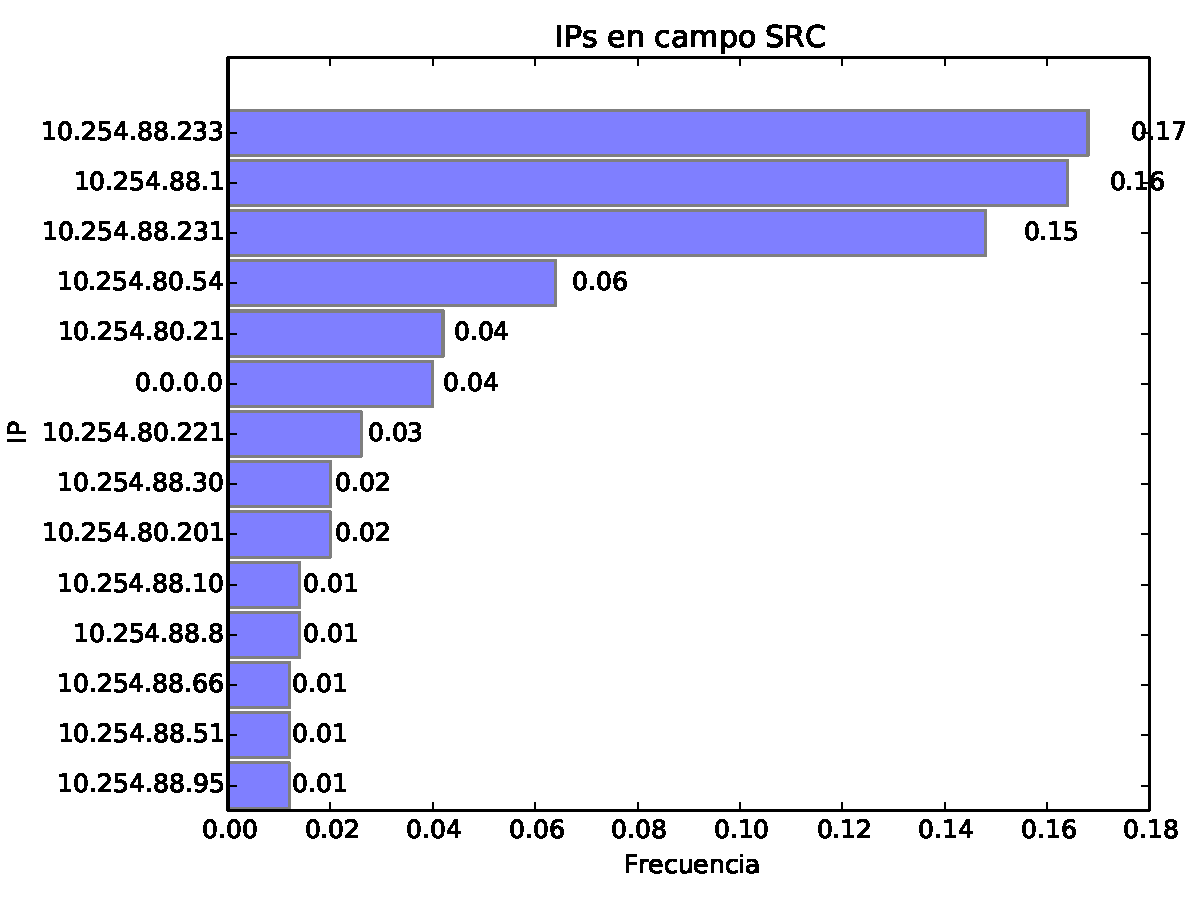
\includegraphics[width=1.0\textwidth]{resultados/starbucks/ipsSrc_4_6187931499.pdf}
		\caption{Estimaci\'on de la probabilidad de cada s\'imbolo en modelo SRC}
	\end{subfigure}
	~
	\begin{subfigure}{0.4\textwidth}
		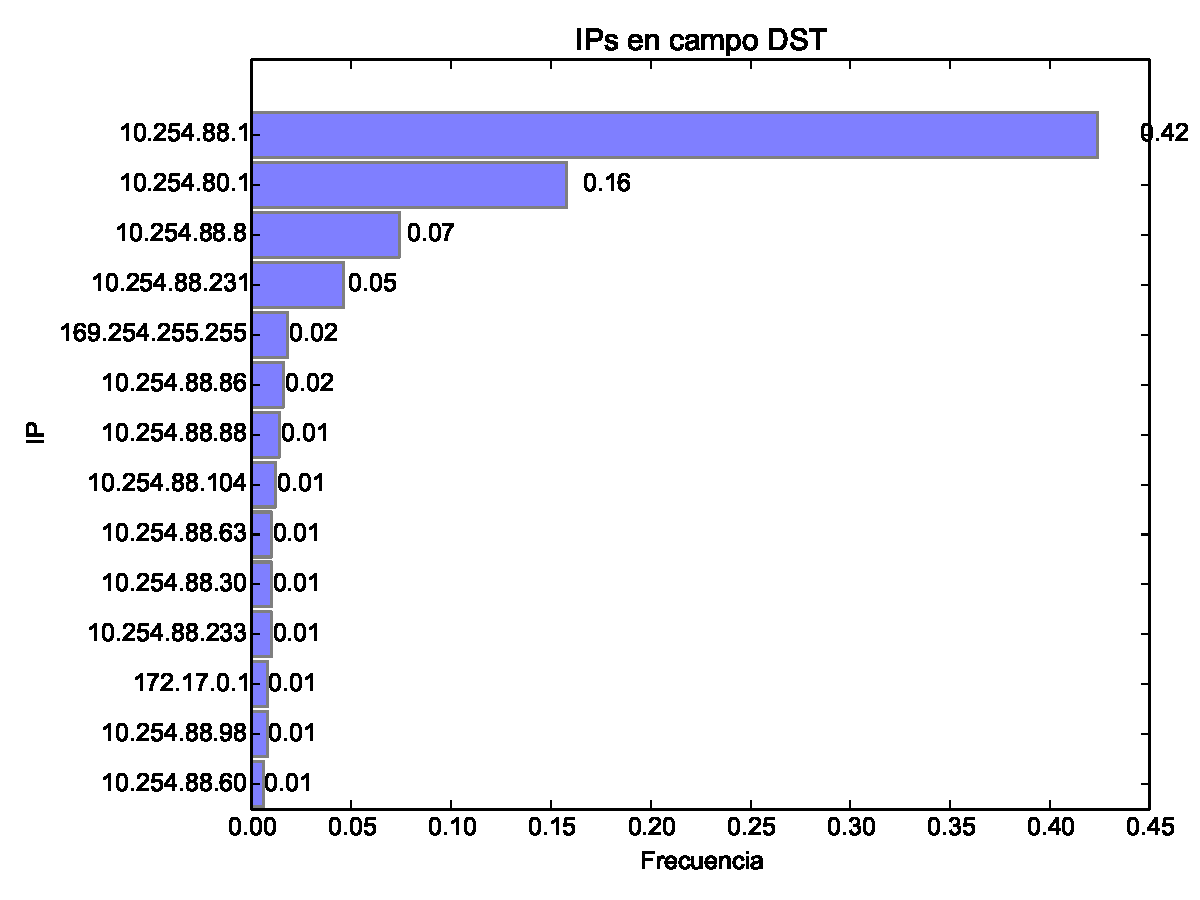
\includegraphics[width=1.0\textwidth]{resultados/starbucks/ipsDst_3_76848714287.pdf}
		\caption{Estimaci\'on de la probabilidad de cada s\'imbolo en modelo DST}
	\end{subfigure}
\end{figure}


\subsection{Empresa}

\begin{wrapfigure}{R}{0.4\textwidth}
\vspace{-35pt}
\hspace{-35pt}
\centering
   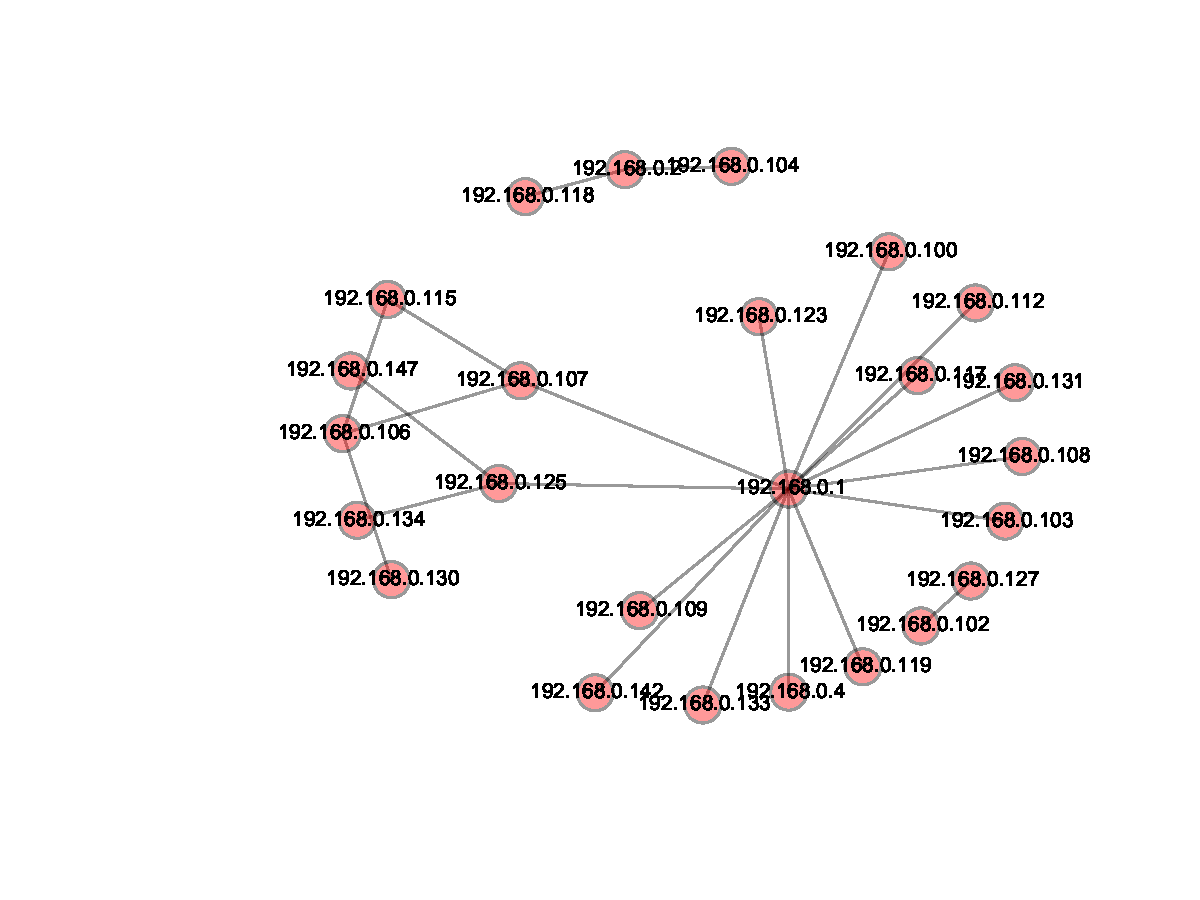
\includegraphics[width=0.4\textwidth]{resultados/empresa/conectividadNX.pdf}
\vspace{-30pt}
   \caption{Topología de la red en una empresa}
\end{wrapfigure}

En este caso la topología del grafo de la red no coincide con la de una estrella. Es posible observar una interacción mucho mayor entre distintos pares hosts, y no únicamente
entre cada uno de estos y el router.

\begin{figure}[H]
	\center
	\begin{subfigure}{0.4\textwidth}
		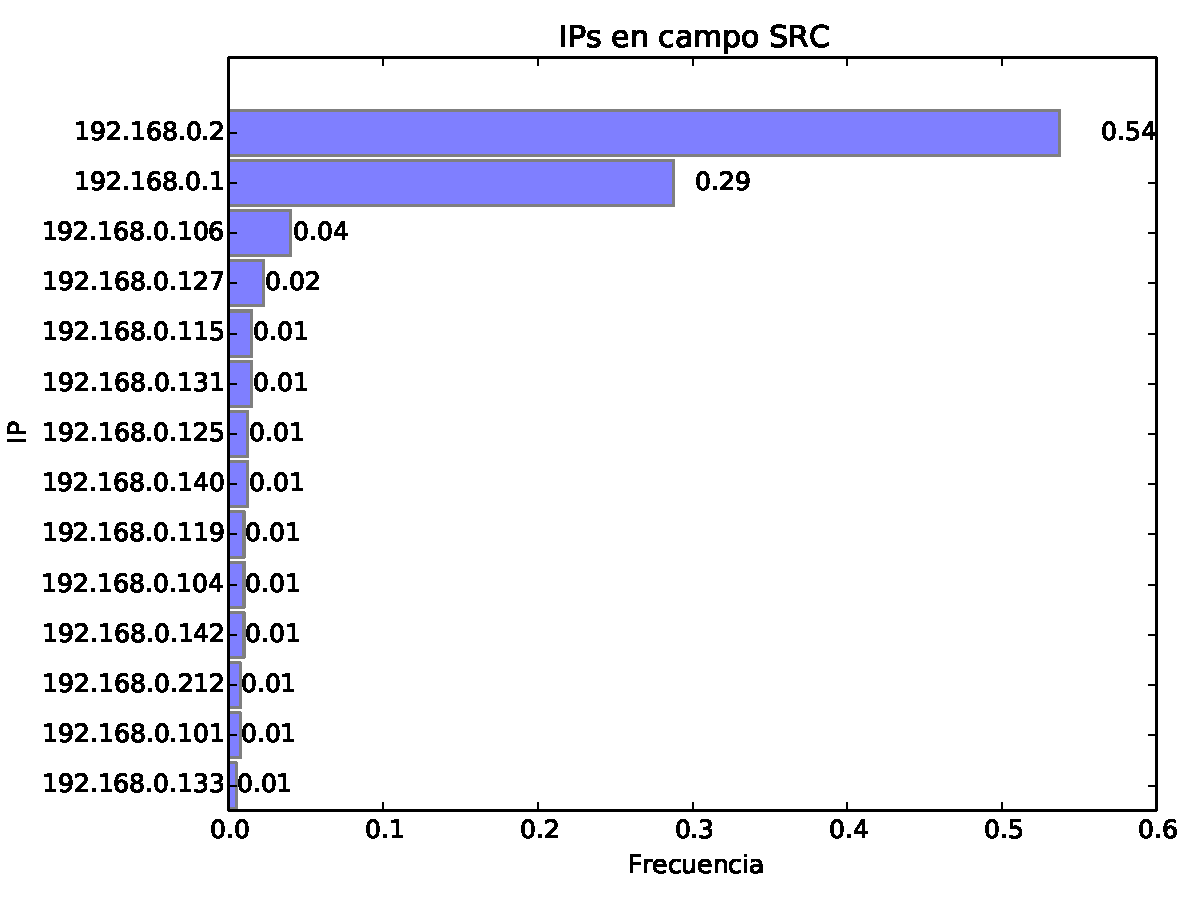
\includegraphics[width=1.0\textwidth]{resultados/empresa/ipsSrc_2_05542931604.pdf}
		\caption{Estimaci\'on de la probabilidad de cada s\'imbolo en modelo SRC}
	\end{subfigure}
	~
	\begin{subfigure}{0.4\textwidth}
		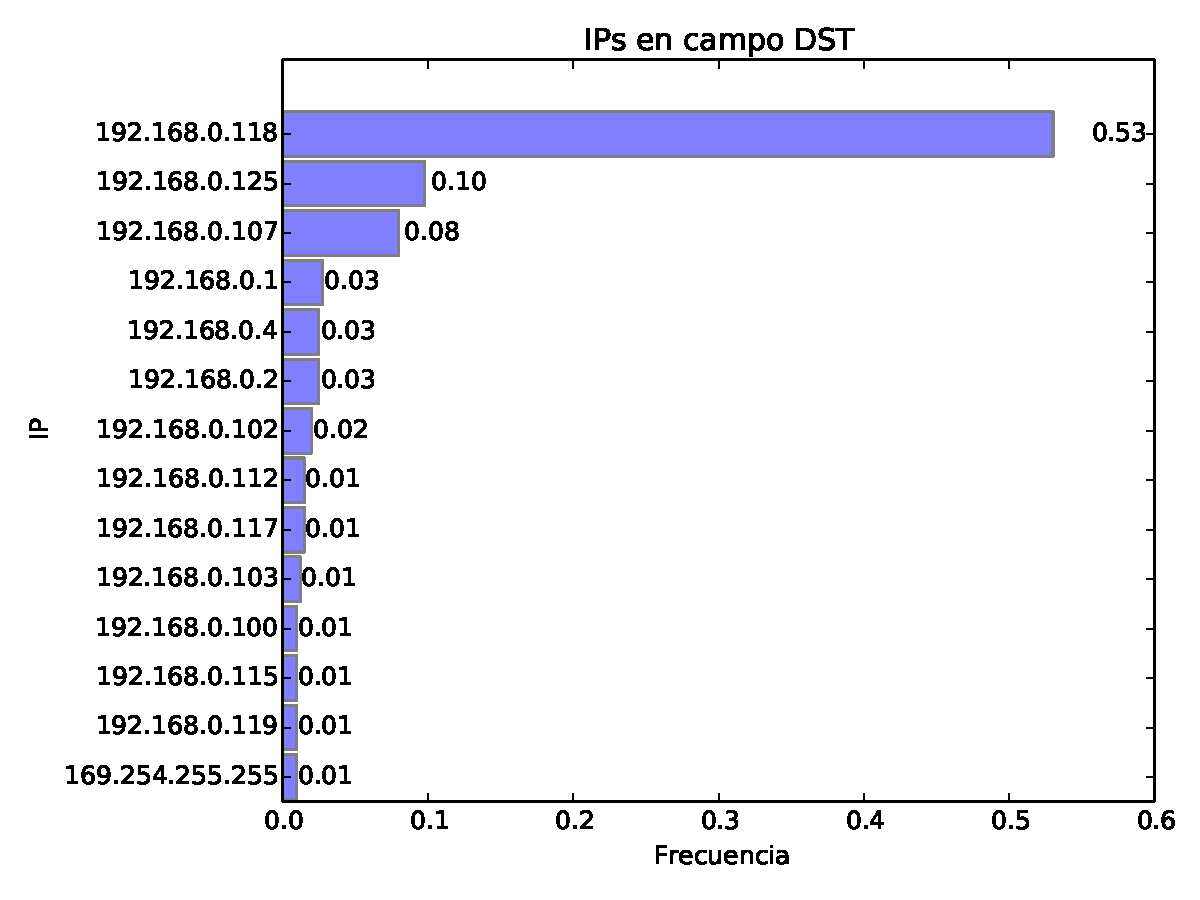
\includegraphics[width=1.0\textwidth]{resultados/empresa/ipsDst_2_99926622579.pdf}
		\caption{Estimaci\'on de la probabilidad de cada s\'imbolo en modelo DST}
	\end{subfigure}
\end{figure}

En el gráfico de barras del modelo SRC el router juega un papel relevante ya que es el segundo símbolo con mayor cantidad de emisión de paquetes. Es interesante mencionar que el 
nodo con mayor cantidad de paquetes enviados, cuya ip es 192.168.0.2, corresponde a un servidor apache. El resto de los nodos que aparecen en el gráfico corresponden a notebooks
y celulares conectados a la red. Este hecho es similar a los experimentos anteriores.

En el gráfico de barras del modelo DST es en donde se nota la mayor cantidad de diferencias. El router no se corresponde con ninguno de los 3 nodos con mayor cantidad de paquetes
recibidos:

\begin{itemize}
    \item 192.168.0.118 corresponde a una notebook
    \item 192.168.0.125 corresponde a un servidor apache
    \item 192.168.0.107 corresponde a un servidor apache
\end{itemize}

Recién aparece en la cuarta posición, con una cantidad de paquetes recibidos considerablemente menor a los primeros. En esta red en particular los dispositivos se envían paquetes
who-has entre ellos en mayor medida, y hacia los servidores en vez de hacia el router.

El valor de la entropía para el gráfico de fuente SRC es $2.05542931604$
El valor de la entropía para el gráfico de fuente DST es $2.99926622579$


~

Los gráficos de barra muestran que el router ha perdido preponderancia respecto a la emisión y recepción de paquetes en comparación con otros nodos distinguidos.

\begin{wrapfigure}{R}{0.4\textwidth}
\vspace{-35pt}
\hspace{-35pt}
\centering
   \includegraphics[width=1\textwidth]{resultados/empresa/conectividad.pdf}
\vspace{-30pt}
   \caption{Grafo de la red}
\end{wrapfigure}

~

\subsection{Entrepiso}

\begin{wrapfigure}{R}{0.4\textwidth}
\vspace{-35pt}
\hspace{-35pt}
\centering
   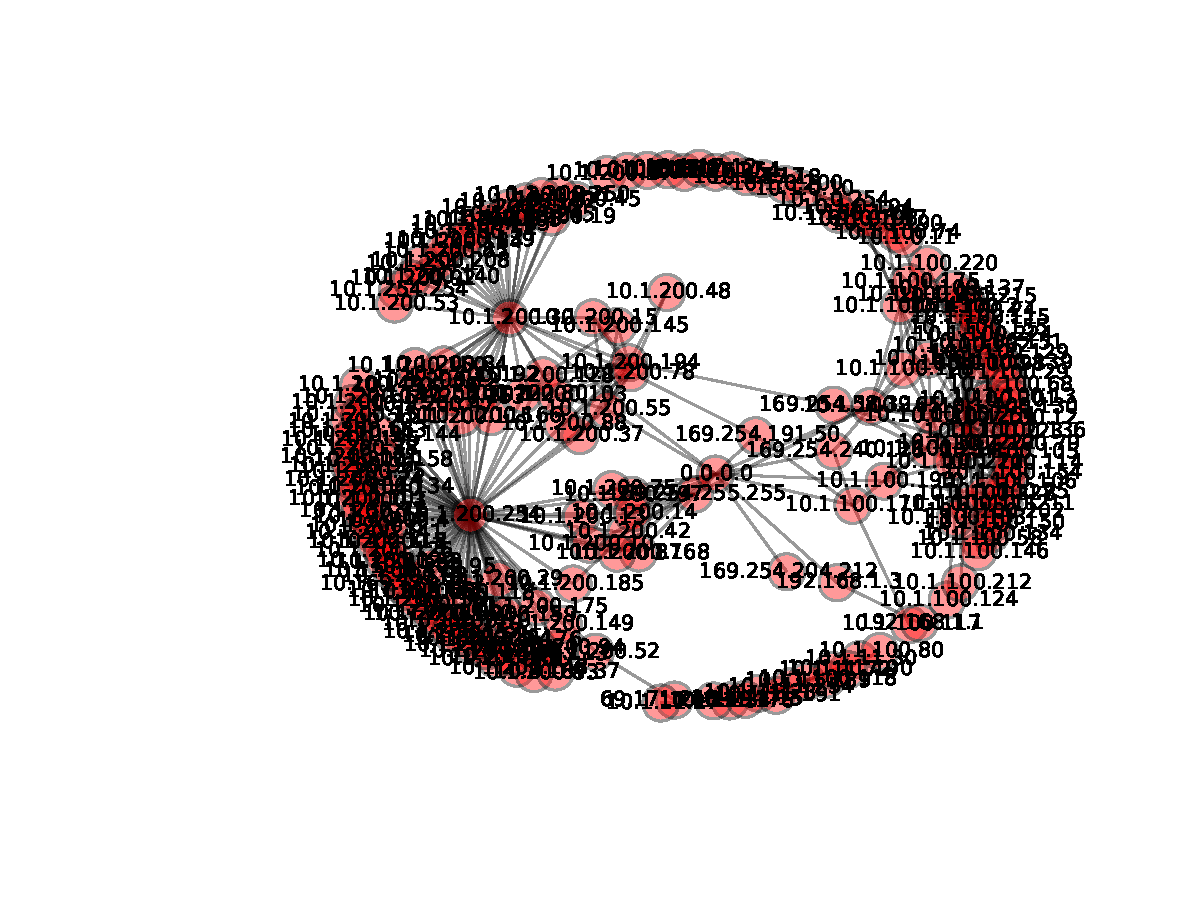
\includegraphics[width=0.4\textwidth]{resultados/entrepiso/conectividadNX.pdf}
\vspace{-30pt}
   \caption{Grafo de la red}
\end{wrapfigure}

En el caso del entrepiso los grafos muestran tres nodos con la forma que caracteriz\'o 
al router dentro de la casa, estos nodos son: 10.1.100.254, 10.1.200.30 y 10.1.200.254.
Sin embargo, estos poseen al menos la mitad de las aparaciones que otros nodos en 
el modelo DST, cosa que $200.30$ repite en SRC. La entrop\'ia fue: $4.25$ para el
modelo $SRC$ y $4.90$ para el modelo DST. El Entrepiso fue la red con mas entrop\'ia.
Una vez mas aparecieron direcciones sueltas, como es por ej: 10.1.11.254.

\begin{figure}[H]
	\center
	\begin{subfigure}{0.4\textwidth}
		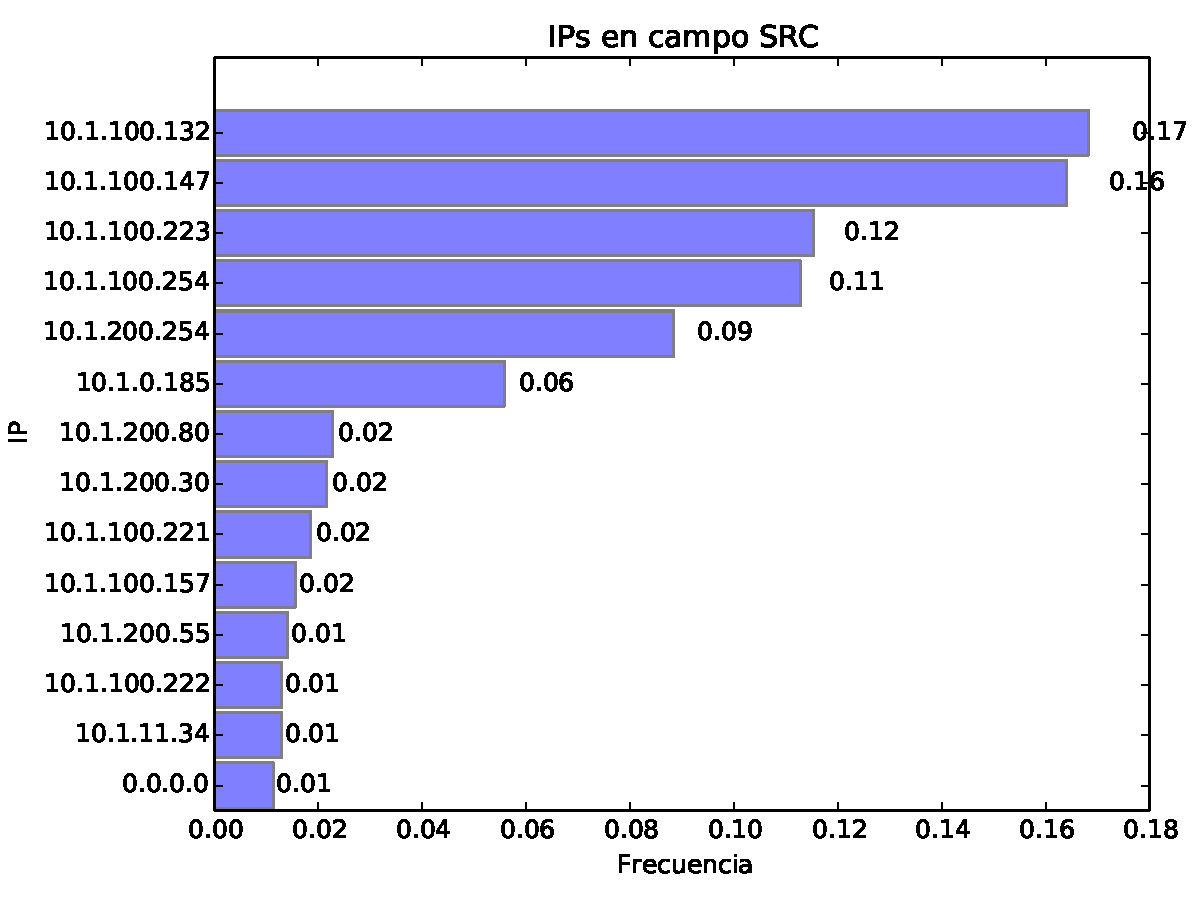
\includegraphics[width=1.0\textwidth]{resultados/entrepiso/ipsSrc_4_25991830161.pdf}
		\caption{Estimaci\'on de la probabilidad de cada s\'imbolo en modelo SRC}
	\end{subfigure}
	~
	\begin{subfigure}{0.4\textwidth}
		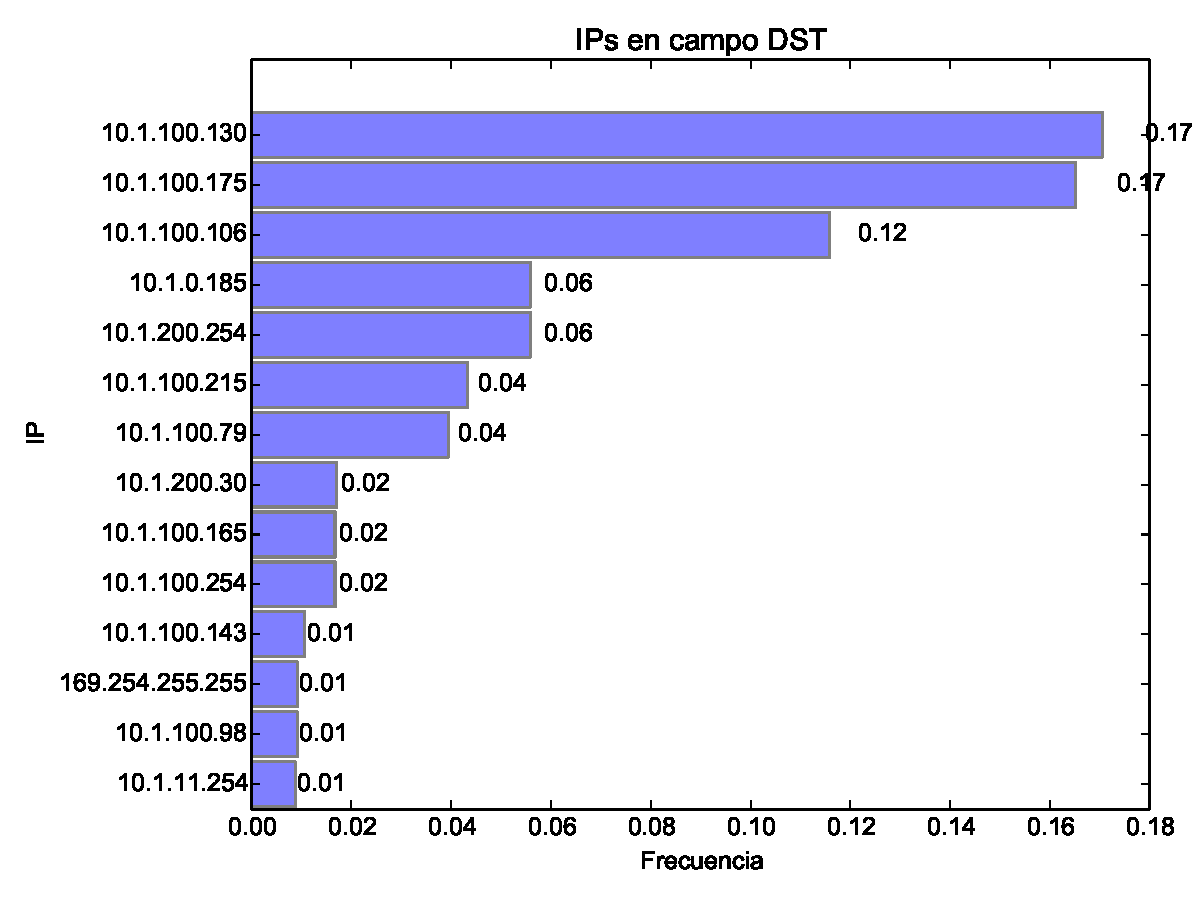
\includegraphics[width=1.0\textwidth]{resultados/entrepiso/ipsDst_4_90633854055.pdf}
		\caption{Estimaci\'on de la probabilidad de cada s\'imbolo en modelo DST}
	\end{subfigure}
\end{figure}

\begin{figure}[H]
	\includegraphics[width=1.0\textwidth]{resultados/entrepiso/conectividad.pdf}
	\caption{Digrafo de conectividad en el entrepiso}
\end{figure}


\subsection{Discusi\'on}

        En todas las redes sucedi\'o que aparecieran direcciones ip que se supone
no pertenecen a la misma. 

        En algunos casos apareci\'o la direcci\'on 169.254.255.255. Investigando
encontramos que es utilizada como broadcast por DHCP que es un protocolo de 
configuraci\'on autom\'atica de par\'ametros de red tales como direcciones IP
para interfaces y servicios.

        La direcci\'on 0.0.0.0 es el estandar para \emph{broadcastear} dentro
de una red local

        Por otra parte, el resto de las direcciones IP que aparecen pueden deberse
a que los routers posean la opci\'on de \emph{Proxy ARP} habilitada, cosa que tiene 
mucho sentido en el caso del Entrepiso por ej.

        A su vez, si bien en los grafos se not\'o claramente la direcci\'on ip
de los routers, esto solo se vio reflejado en la estimaci\'on de la probabilidad
en los modelos solo en la Casa y el Starbucks. Esto muestra que el contar la 
cantidad de apariciones de una IP en los campos no es suficiente para detectar
los routers de la red.

        Por otra parte, ser\'ia interesante realizar otro experimento para ver
si las direcciones con mayor frecuencia de aparici\'on se corresponden a dispositivos
utilizados durante largos per\'iodos dentro de la red. Quizas esto permite detectar
los nodos utilizados por usuarios.  ESTO REFORZARLO O TIRARLO ABAJO EN BASE AL 
CONOCIMIENTO DEL LUGAR DE TRABAJO... EN CASO DE NO SABER, MENTIR.


